\chapter{Element of Room Acoustics}\label{chap:acoustics}

\newthought{Synopsis} This chapter will cross an important bridges: from the physics to analog signal processing
Acoustics is basically how sounds works in environment.


\section{Sound Wave Propagation}

Sound is a complex concept and complex concepts creates theories.


from https://plato.stanford.edu/entries/sounds/
The main relevant families of answers include proximal, medial, distal, and aspatial theories.
Proximal theories would claim that sounds are where the hearer is.
Medial theories—exemplified by mainstream acoustics—locate sounds in the medium between the resonating object and the hearer.
Distal theories consider sounds to be located at the resonating object. Finally, aspatial theories deny spatial relevance to sounds.

What is the definition? The etymology?
How is it perceived, how is it measured? How is it represented?

speed of sound

\begin{equation}
    \cair =  331.4 + 0.6\temperature + 0.0124\rhumidity \; \text{m/s}
    .
\end{equation}


If we think at the process of sound production in the light of the classic \textit{source-medium-receiver} model of communication theory,
we can say that in we have studied models for the source of sound signals. We now move a step further and examine the effects of the medium in which sound propagates, and the receiver, specifically a human receiver with two ears.

Equation are reproduced or modified from \cite{Kuttruff2009room, Marczuk2006modelling, Habets2010generator, Avanzini2019Chapter4, Allen1999image}

When vibrating objects excites air, molecules that start oscillating creating local pressure deviation from the atmospheric pressure.
Such vibration of of air molecules takes place in the direction of the excitement, with the next layer of molecules excited by the first layer.
The molecules oscillate in the frequency of the initial exciting vibration, creating oscillating of higher and lower density of molecules.
Pushing layer by layer forward, a \textit{longitudinal} wave is created.
% \marginpar{%
    % \animategraphics[loop,autoplay]{12}{./figures/general/Lwave-}{0}{50}
% }

Sound is mechanical energy in the form of pressure variances in an elastic medium. These pressure variances propagate as waves from a vibrating source.

Changes in air pressure (air being a propagating medium) can be represented by a WAVEFORM, which is a graphic representation of a sound. In reality, sound waves propagate through the air in LONGITITUDAL WAVES (and not TRANSVERSE WAVES):

\subsection{The Acoustic wave equation}
\label{subsec:acoustics:waveq}

The \textit{acoustic wave equation} governs the propagation of acoustic waves through a perfectly elastic medium (gas or liquid) in a 3D space.
The equation describes the evolution of acoustic pressure $\pressure$ as function of the position $\positionSource$ $[\si{\metre}]$ and time $t$ $[\si{\second}]$
\marginpar{%
    The symbol $\knabla^2 = \kpderiv[2]{}{x} + \kpderiv[2]{}{y} + \kpderiv[2]{}{z}$
    stands for the 3-dimensional \textit{Laplacian} operator.
}
\begin{equation}
    \label{eq:acoustics:wave}
    \knabla^2 \pressureSpaceTime - \frac{1}{\speedOfSound^2} \kpderiv[2]{\pressureSpaceTime}{t} = 0
    .
\end{equation}
The constant $\speedOfSound$ is the sound velocity in the medium with dimension $\frac{\si{\metre}}{\si{\second}}$.

As opposed to mechanical vibrations in a string or (drum) membrane, acoustic vibrations are \textit{longitudinal} rather than \textit{transversal},
\ie/ the air particles are displaced in the same direction of the wave propagation.
\marginpar{%
    In 1746, d’Alembert discovered the one-dimensional wave equation for music strings,
    and within ten years Euler discovered the three-dimensional wave equation for fluids.
}

Assuming the propagation of the wave in a homogeneous medium, one can obtain the equation above by combining three fundamental physical laws:
\begin{itemize}
    \item the \textit{conservation of momentum}\sidenote{its appliction to fluids comes with the name of the Euler's equation},
    \item the \textit{conservation of mass} (\aka/ the continuity equation), and
    \item the \textit{equation of state} (\aka/ the gas law)
\end{itemize}
In case of inhomogeneous medium, scalar inhomogeneities, \eg/ due to temperature variation,
and vector inhomogeneities, \eg/ due to presence of fans or air conditioning
brakes the underlying assumption of the model.
However these effect are typically small in typical application of speech and audio signal processing.
Thus they are commonly ignored.

\newthought{The Derivation of}~\cref{eq:acoustics:wave} starts by considers a infinitesimal volume unit $V$ of a fluid or gas (such as air), whose center of gravity is located at $\positionMicrophone$.
Let $\mass$ be the mass of such volume.
By the well-known Newton's second law, applying a force $F$ to the fluid, its acceleration increase proportionally to $\mass$,
namely:
\begin{equation}
    \label{eq:acoustics:newton}
    \forceVec = \mass \kpderiv[]{\velocity\depSpaceTime}{t}
\end{equation}
\marginpar{%
Newton's Law II: The alteration of motion is ever proportional to the motive force impress'd;
and is made in the direction of the right line in which that force is impress'd.
\\Orignal: \emph{Lex II: Mutationem motus proportionalem esse vi motrici impressae,
et fieri secundum lineam rectam qua vis illa imprimitur.}
}
where $\velocity(\positionSource, t)$ denotes the volume velocity and $t$ the time $[\si{\second}]$.
The force can be expressed in terms of difference of acoustic pressure $p$ at $\positionMicrophone$ on a surface of the volume, $\surface$, namely
\begin{equation}
    \label{eq:acoustics:pressure}
    \forceVec = - V \kbracket{\kgrad{\pressureSpaceTime}}
\end{equation}
where $\kgrad{}$ is is the gradient operator.
By combining \cref{eq:acoustics:newton,eq:acoustics:pressure}, we obtain the famous \textit{Euler's equation of motion}:
\begin{equation}
    \label{eq:acoustics:euler}
    \kgrad{\pressureSpaceTime} = - \densityEq \kpderiv[]{\velocity\depSpaceTime}{t}
\end{equation}
where $\densityEq = \frac{\mass}{\surface}$ is the static density of the medium
\footnote{%
\label{fn:acoustics:airconstanc}
\\Air Denisity $\density_{\text{air}} = 1.18 \tfrac{\si{\kilogram}}{\si{\metre^3}}$.
\\Air Gas constant $R_{\text{air}} = 286.9 \tfrac{\si{\joule}}{\si{\kilogram} \si{\mole}}$.
\\Air Adiabatic index $\gamma_{\text{air}} = 1.4$.
\\Speed of sound in air $\speedOfSound_{\text{air}} = 343.1 \tfrac{\si{\metre}}{\si{\second}}$.
}.

\newthought{Secondly, by the Conservation of Mass} principle,
the total mass must remain constant as the it is in a deformable medium. This principle
translates into the \textit{continuity equation}, written in the differential form:
\begin{equation}
    \label{eq:acoustics:continuity}
    \kpderiv[]{\eta\depSpaceTime}{t} = V \kbracket{\divergence{\bfq\depSpaceTime}}
\end{equation}
where
\begin{itemize}
    \item $\eta\depSpaceTime$ is the the amount of the quantity q per unit volume
    \item $\eta\depSpaceTime$ is the volume variation due to the pressure changing
\end{itemize}
inside the volume $\volumeUnit$ in time is equal to the total amount of mass passing thought the surface .

\newthought{Finally, the State Equation} describes the properties of the propagation medium.
Assuming that the fluid (or gas) to be ideal, the \textit{Charles-Boyle} gas law states\sidenote{The original gas law writes $P V = n R T$. Here the law is written in terms of \textit{specific volume}}
\begin{equation}
    P V = R T
\end{equation}
where $P$ is the total pressure on the volume $V$; $T$ the absolute temperature in degrees Kelvin and $R$ is specific gas constant\cref{fn:acoustics:airconstanc}.
The dependency upon space and time $\depSpaceTime$ is here omitted for sake of compactness and readability.

Since the exchange of heat of wave of acoustic frequencies range in negligible, the whole process can be considered thermodynamically \textit{adiabatic}.
In such scenario, the relation between the total pressure and the volume is given by
\begin{equation}
    \label{eq:acoustics:state}
    P V^\gamma = \const
\end{equation}
where $\gamma$ is the adiabatic index of the medium~\cref{fn:acoustics:airconstanc}.

The total pressure and the total volume consist in a sum of a constant and a variable term, that is $P = P_0 + p$, $V = V_0 + \nu$ respectively.
Considering that $p \ll P_0$ and $\nu \ll V_0$, the time-differential of~\cref{eq:acoustics:state} with respect to time reads
\begin{equation}
    \label{eq:acoustics:statediff}
    \kpderiv[]{\pressureSpaceTime}{t} = - \gamma \frac{P_0}{V_0} \kpderiv[]{\nu\depSpaceTime}{t}
\end{equation}

\newthought{Finally, the Acoustic Wave Equation} can be now derived by combining together
the equation of motion~\ref{eq:acoustics:euler},
the continuity equation~\ref{eq:acoustics:continuity},
and the state equation~\ref{eq:acoustics:statediff}.
In particular the combination of~\cref{eq:acoustics:continuity,eq:acoustics:statediff},
\begin{equation}
    \kpderiv[]{\pressureSpaceTime}{t} = - \gamma P_0 \kbracket{\divergence{\bfq\depSpaceTime}}
    ,
\end{equation}
can be differentiated with respect to time $t$ yielding to
\begin{equation}
    \kpderiv[2]{\pressureSpaceTime}{t} = - \gamma P_0 \kbracket{\divergence{\kpderiv[]{\bfq\depSpaceTime}{t}}}
    .
\end{equation}
Taking the divergence of each side of the~\cref{eq:acoustics:euler}, we get
\marginpar{%
The \textit{Laplacian} of a function is the given by the divergence of the gradient of that function,
\\in math $\knabla^2 x = \divergence{\kgrad{x}}$}
\begin{equation}
    \knabla^2 \pressureSpaceTime = -\densityEq \kbracket{\divergence{q\depSpaceTime}}
\end{equation}
The above two equation can be combined leading to
\begin{equation}
    \knabla^2 \pressureSpaceTime = \frac{1}{\speedOfSound^2} \kpderiv[2]{\pressureSpaceTime}{t}
\end{equation}
where the $\speedOfSound$ is the speed of sound and is related to the medium properties through
\begin{equation}
    \speedOfSound^2 = \frac{\gamma P_0}{\densityEq}
    .
\end{equation}


\newthoughtpar{The Helmholtz's equation}
The wave equation~\ref{eq:acoustics:wave} is expressed in the space-time domain $\depSpaceTime$.
By applying the temporal Fourier transform to the wave equation we obtain the time-independent \textit{Helmholtz equation} is obtained, \ie/
\begin{equation}
    \label{eq:acoustics:helmholtz}
    \knabla^2 P(\positionMicrophone, f) + k^2 P(\positionMicrophone, f) = 0
    ,
\end{equation}
where $k \frac{2 \pi f}{c}$ denotes the \textit{wave number}, that relates the frequency $[\si{\hertz}]$ and the propagation velocity.

The wave equation~\ref{eq:acoustics:wave} and the Helmholtz's equation~\ref{eq:acoustics:helmholtz} are source independent,
namely no source is present in the medium. Therefore they called \textit{homogeneous} as the right-hand term are zero.

Normally the sound field is a complex field generated by multiple acoustics sources. As consequence, the two equation becames
inhomogeneous as some non-zero terms needs to be added to the right-hand sides.
\todo{cite [27]}

In presence of a sound source producing waves with distribution function $s(t, \positionSource)$, the wave equation can be written
\begin{equation}
    \label{eq:acoustics:source}
    \knabla^2 \pressureSpaceTime - \frac{1}{\speedOfSound^2} \kpderiv[2]{\pressureSpaceTime}{t} = s(t, \positionSource)
    .
\end{equation}
Then, the correspondent Helmholtz's equation writes
\begin{equation}
    \label{eq:acoustics:source_freq}
    \knabla^2 P(\positionMicrophone, f) + k^2 P(\positionMicrophone, f) = - S(\positionSource, f)
    .
\end{equation}

For instance one can assume an infinitesimally small pulsating sphere locate at $\positionSource$ radiating constant acoustic energy at frequency $f$.
For the receiver position $\positionMicrophone \neq \positionSource$, the Helmholtz's equation writes

\begin{equation}
    \label{eq:acoustics:green_definition}
    \knabla^2 H(f, \positionMicrophone \mid \positionSource)
     + k^2 H(f, \positionMicrophone \mid \positionSource) = - \delta(\positionMicrophone - \positionSource)
    ,
\end{equation}
where the term $H(f, \positionMicrophone \mid \positionSource)$ is an \textit{Green's function}.
For the properties of the Green's functions, $H(f, \positionMicrophone \mid \positionSource)$ is also solution of the homogeneous Helmholtz equation~\ref{eq:acoustics:helmholtz}.
The source is describe here by $\delta(\positionMicrophone - \positionSource)$, which in this context is a 3-dimension Dirac function.
We will see in the next subsection that the function $H$ solving~\ref{eq:acoustics:green_definition} can be interpreted as the free-field \textit{Transfer Function}
between the source at $\positionSource$ and the receiver at $\positionMicrophone$.

\subsection{... and its solution as Green's function}
\textsc{The Green's Functions} are mathematical tools for solving linear differential equations with specified initial- and boundary- condition \cite{Duffy2015}.
\marginpar{%
\footnotesize
By 1950 Green’s functions for Helmholtz’s equation were used to find the
wave motions due to flow over a mountain  and in acoustics.
Green’s functions for the wave equation lies with Gustav Robert Kirchhoff (1824–1887),
who used it during his study of the three-dimensional wave equation.
He used this solution to derive his famous \textit{Kirchhoff’s theorem}.
\\--- Duffy, 2015.
}
They have been used to solve many fundamentals equation, among which \cref{eq:acoustics:helmholtz,eq:acoustics:wave} for both free and indoor propagation.
They can be seen as the equivalent concept of the \textit{impulse responses} (\resp/ transfer function) used in signal processing.
Under this light and by assuming the fluid  medium as the \textit{linear filter}, the physic so-far can be rewritten in the vocabulary of
the communication theory, namely \textit{input}, \textit{filter} and \textit{output}.

Green say that the partial differential equations above can be solved for arbitrary source as follows:

\begin{equation}
    \label{eq:acoustics:helmholz_conv}
    P(f, \positionMicrophone) = \iiint_{\volume_\contSource} H(f, \positionMicrophone \mid \positionSource) S(f, \positionSource) \kdiff\positionSource
    ,
\end{equation}
where $\volume_\contSource$ denotes the source volume,
and  $\kdiff\positionSource =  \kdiff{x_\contSource}\,\kdiff{y_\contSource}\,\kdiff{z_\contSource}$ the  differential  volume element at position $\positionSource$.

It can be shown \cite{Kutruff} that the time-invariant Green's function for~\cref{eq:acoustics:helmholtz,eq:acoustics:green_definition} writes
\begin{equation}
    \label{eq:acoustics:greenFreeFreq}
    H(f, \positionMicrophone \mid \positionSource) = - \frac{1}{4 \pi \norm{\positionMicrophone - \positionSource}} e^{- \frac{\Ii 2 \pi f \norm{\positionMicrophone - \positionSource}}{\speedOfSound}}
\end{equation}
where $\norm{\cdot}$ denotes the Euclidean norm.
\\By applying the inverse Fourier transform to the result above, we can write the time-domain Green's function as
\begin{equation}
    \label{eq:acoustics:greenFreeTime}
    h(t, \positionMicrophone \mid \positionSource) =
        - \frac{1}{4 \pi \norm{\positionMicrophone - \positionSource}}
        \diracOf{t - \frac{\norm{\positionMicrophone - \positionSource}}{\speedOfSound}}
\end{equation}
where $\diracOf{\cdot}$ is the time-directional Dirac delta function.
This corresponds to a pure impulse at time $t = \tfrac{\norm{\positionMicrophone - \positionSource}}{\speedOfSound}$,
\ie/ the propagation time from $\positionSource$ to $\positionMicrophone$.

\newthought{Finally,} the initial sound pressure $\pressureSpaceTime$ can now be computed by taking the frequency-directional inverse Fourier transform of \cref{eq:acoustics:helmholz_conv}.
\todo{from this to convolution}


% \newthought{The Conservation of Momentum}

% \marginpar{%
% \footnotesize
% Law I: Every body persists in its state of being at rest or of moving uniformly straight forward,
% except insofar as it is compelled to change its state by force impressed.
% \\Newton's original Latin reads: \emph{Lex I: Corpus omne perseverare in statu suo quiescendi vel movendi uniformiter in directum,
% nisi quatenus a viribus impressis cogitur statum illum mutare}}

% 2nd Newton law
% \sidenote{%
% Law II: The alteration of motion is ever proportional to the motive force impress'd;
% and is made in the direction of the right line in which that force is impress'd.
% \\Orignal: \emph{Lex II: Mutationem motus proportionalem esse vi motrici impressae,
% et fieri secundum lineam rectam qua vis illa imprimitur.}}

% \begin{equation}
%     F = m a
% \end{equation}

% \begin{equation}
%     F = \kgrad{\pressure}
% \end{equation}
% $\kgrad$ denotes the three-dimensional gradient with, namely respect to space.

% 3nd Newton law and Conservation of momentum
% \sidenote{%
% Law III (action-reaction law): To every action there is always opposed an equal reaction:
% or the mutual actions of two bodies upon each other are always equal, and directed to contrary parts
% \\Original: \emph{Lex III: Actioni contrariam semper et æqualem esse reactionem:
% sive corporum duorum actiones in se mutuo semper esse æquales et in partes contrarias dirigi.}}
% writes
% \begin{equation}
%     \label{eq:acoustics:momentum}
%     \kgrad{\pressure} = - \mass \kpderiv[]{\bfv}{t} = - \volumeUnit \kpderiv[]{\bfv}{t}
% \end{equation}
% where the mass $\mass$ is substituted by the density per unit volume $\volumeUnit$ since the unit of volume $V$ is considered as reference.

% Evolution of sound pressure $\pressure \depSpaceTime$
% as a function of position $\positionMicrophone = \klist{x, y, z}$ $[\si{\metre}]$ and time $t$ $[\si{\second}]$.

% \newthought{Conservation of Mass}
% \sidenote{Nothing comes from noting. In latin \textit{nihilo nihil fit} ---Parmenide}

% In the field of fluid and continuous mechanics, the this law can be formulated mathematically using the \textit{continuity equation} in \textit{differential form}:
% \begin{equation}
%     \kpderiv[]{\rho}{t} + \kdivergence{\kparen{\rho \bfv}} = 0
%     ,
% \end{equation}
% where $\rho$ is the density (mass per unit volume).


% \begin{equation}
%     \kpderiv[]{\eta}{t} + \eta_0 \kdivergence{\bfv} + = 0
%     ,
% \end{equation}

% Considering the same unit of volume $V$, the conservation of mass law states that in a system that does not exchange
% neither energy nor mass with the surrounding environment, the mass remains constant.
% This is equivalent to say that the variation of mass inside $V$ is equal to the the amount of mass passing thought its volumetric surface, namely:


% where $\knabla\cdot$ is the divergence operator, $\eta$ is the density (mass per unit volume) and $\bfv$ is flow velocity field.
% where $\eta = \eta_0 + \Delta\eta$ is the total density within the volume accounting for the a static part $\eta_0$ and a variable part $\Delta\eta$.

% The interpretation of the continuity equation for mass is the following: For a given closed surface in the system,
% the change in time of the mass enclosed by the surface is equal to the mass that traverses the surface, positive if matter goes in and negative if matter goes out

% By dividing the momentum conservation law in \cref{eq:acoustics:momentum} and differentiating both members with respect to space, it becomes:
% \begin{equation}
%     \kpderiv[]{}{t} \knabla\cdot \bfv = - \frac{1}{\volumeUnit} \knabla^2 p
% \end{equation}



% \marginpar{
%     $\knabla^2 = \kpderiv[2]{}{x} + \kpderiv[2]{}{y} + \kpderiv[2]{}{z}$
%     is the \textit{Laplacian} expressed  in  the  Cartesian  coordinates $\klist{x, y, z}$.
% }
% \begin{equation}
%     \label{eq:acoustics:wave}
%     \kpderiv[2]{\pressureSpaceTime}{t} = \cair^2 \knabla^2 \pressureSpaceTime
%     ,
% \end{equation}
% where $\cair$ is the speed of sounds.

% This equation is accurate as long as the sound field $\abs{\pressureSpaceTime} \ll \densityEq \cair^2$
% where $\densityEq$ is the density of the propagation medium at equilibrium. It is not true when
% \begin{itemize}
%     \item scalar inhomogeneities (spatial distribution of sound speed or air density): temperature variation in the medium
%     \item vector inhomogeneities (spatial distribution of particle mean velocity): presence of fans or air conditioning
% \end{itemize}
% In room acoustics this effects are too small, hence typically ignored.

% Sound field from a source in a specific room, we need the source function and boundary condition that describes the sound reflection and absorption at the walls.
% \begin{equation}
%     \label{eq:acoustics:wave}
%     \kpderiv[2]{\pressureSpaceTime}{t} - \cair^2 \knabla^2 \pressureSpaceTime = - \contSource\depSpaceTime
%     ,
% \end{equation}
% where $\contSource\depSpaceTime$ denote the source function \cite{Room Impulse Response Generator, Habets}

% By applying the Fourier Transform to \cref{eq:acoustics:wave}, we obtain the time-independent Helmholtz equation
% \sidenote{\textbf{Helmholtz equation:} In mathematics, it is referred to the eigenvalue problem for the laplacian operator, that is.
% $\knabla^2 f = - k^2 f$.  where $k$ is the eigenvalue, called \textit{wave number} in case of waves, and $f$ in the (eigen)function, \textit{amplitude} in case of wave.}:
% \begin{equation}
%     \knabla^2 P(\positionMicrophone ; f) + k^2 P(\positionMicrophone ; f) = 0
% \end{equation}
% where $k = \sfrac{2 \pi f}{\cair}$ is the \textit{wave number}, function of frequency $f$ and


% In presence of a harmonic source producing waves described by the function $s(\positionMicrophone ; f)$, the propagation of its acoustic
% signal (small amplitude, ideal (non-viscous)) in a fluid medium my be described by the following \textit{linear}, lossless, non-homogeneous wave equation
% \begin{equation}
%     \label{eq:acoustics:helmholtzSource}
%     \knabla^2 p(t, \positionMicrophone) + \frac{1}{\cair^2} \kpderiv[2]{\pressureSpaceTime}{t} = s(t, \positionMicrophone).
% \end{equation}

% Threating the fluid medium as a \textit{linear filter}, this equation may be solved taking advantages of the signal and system theory.
% We get the alternative solution to this problem (as compared with the conventional approach).

% In the typical signal and system theory, the relation between the input (source) $x(t, \positionSource)$ and
% the output $y(t', \positionMicrophone)$ is described by the following relation:

% \begin{equation}
%     \label{eq:acoustics:lti}
%     y(t', \positionMicrophone) =
%     \int \int
%         h(t \kto  t' ; \positionSource \kto \positionMicrophone)
%         x(t, \positionSource)
%         \kdiff t  \kdiff \positionSource
% \end{equation}

% where $h(t \kto  t' ; \positionSource \kto \positionMicrophone)$ is the \textit{impulse response} of the linear filter, namely the response of the system
% in the point with coordinates $\positionMicrophone$ at the time $t'$, if the unit-amplitude impulse was applied at the input at the time $t$ and location $\positionSource$.

% By considering now the generic source function $s(t, \positionSource)$ as input function of the linear system and considering the pressure variation $\pressure$ as the output of the system,
% we can rewrite \cref{eq:acoustics:lti} as follows:

% \begin{equation}
%     \label{eq:acoustics:lti:pressure}
%     p(t', \positionMicrophone) =
%     \int \int
%         h(t \kto  t', \positionSource \kto \positionMicrophone)
%         s(t, \positionSource)
%         \kdiff t  \kdiff \positionSource
% \end{equation}
% The function $h(t \kto  t', \positionSource \kto \positionMicrophone)$ is the impulse response (Green's function)
% along the transmission path between the source point $\positionSource$ and the receiver point $\positionSource$.

% By applying the Fourier transform to both sides of equation \cref{eq:acoustics:helmholtzSource}, we obtain:
% \begin{equation}
%     \label{eq:acoustics:helmholtzSource}
%     \knabla^2 P(f, \positionMicrophone) + \kparen{2 \pi f / \cair}^2 P(f, \positionMicrophone) = S(f, \positionMicrophone).
% \end{equation}

% where  $P(f, \positionMicrophone)$ is the Fourier transform of the pressure $\pressure$ and $f$ in the frequency in $\si{\hertz}$.

% In the frequency domain, eq.~\cref{eq:acoustics:lti:pressure} writes

% \begin{equation}
%     P(f, \beta) = H(f, \beta) S(f, \beta)
% \end{equation}


% If a unit-amplitude harmonic point source at position $\positionSource$, $S(\positionMicrophone ; f) = \delta(\positionMicrophone - \positionSource)$,
% where $\delta$ is the Kronecker delta function defining a point in the space.
% The partial differential equation \cref{eq:acoustics:helmholtzSource} can be solved by first solving the following inhomogeneous equation:
% \begin{equation}
%     \knabla^2 G(\positionMicrophone ; f) + k^2 G(\positionMicrophone ; f) = - \delta(\positionMicrophone - \positionSource)
% \end{equation}

% where the the solution $G(\positionMicrophone ; f)$ is called \textit{Green's function}.

% \subsection{The Green's Function as solution of the Wave Equation}

% Why do we use Green's functions?
% \cpother{Using the Green theorem, the integrated equation may be constructed,
% linking the effect of action of the source, wave propagation,
% boundary and initial conditions in the simple formula.}

% Green's functions
% \begin{itemize}
%     \item used to solve initial- and boundary-value problems, involving differential equations [Duffy, 15]
%     \item defined as impulse responses of homogeneous systems
% \end{itemize}
% Thus they are used to solve the sound wave equation for indoor propagation.

% The solution of equation eq.~\cref{eq:acoustics:helmholtzSource} can be expressed in term of \textit{bundary conditions},
% \textit{initial conditions} and the \textit{Green's function} $g$.
% Such function is found by solving

% \begin{equation}
%     \knabla^2 g + \frac{1}{\cair^2} \kpderiv[2]{g}{t} = - \delta(\positionMicrophone - \positionSource)\delta(t - t_0)
% \end{equation}
% where $\positionSource$ is the position of the source.
% This equation describes the effect of an impulse as it propagates from $\positionMicrophone=\positionSource$ as time increases form $t = t_0$.



% The Green's function $g({\positionMicrophone}_0, t_0, \positionMicrophone, t)$ is then the solution to the wave equation

% As in Duffy: Acoustic wave equation defined in \cref{eq:acoustics:wave}, can be rewritten
% \begin{equation}
%     \kderiv{2}{g}{t}
% \end{equation}

% The solution of the Helmholtz equation, describing the propagation of a wave in the free space
% The Green's function for a free (unbounded) space for an omnidirectional point sources is
% \begin{equation}
%     G(f, \positionMicrophone \mid \positionMicrophone = - \frac{1}{4 \pi \norm{\positionMicrophone - {\positionMicrophone}_0}} e^{- \frac{\Ii  2 \pi f \norm{\positionMicrophone - {\positionMicrophone}_0}}{\cair}}
% \end{equation}

% The inverse Fourier Transform
% \begin{equation}
%     g(t, \positionMicrophone \mid \positionMicrophone = - \frac{1}{4 \pi \norm{\positionMicrophone - {\positionMicrophone}_0}} \delta \kparen{t - \frac{\norm{\positionMicrophone -{\positionMicrophone}_0}}{\cair}}
% \end{equation}

% The Green's function for the sound wave equation will be here derived here:

%%%%%%%%%%%%%%%%%%%%%%%%%%%%%%%%%%%%%%%%%%%%
\section{Acoustic Reflections}

\todo{From Schimmel's paper, Kutruff and Remaggi}

% The acoustic reflection are the main object of this thesis.
The equations derived so far assumed unbounded medium, \ie/ free space: a rare scenario in everyday applications.
Real mediums are bounded, limited, at least partially.
For instance for the sound (wave) in a room, the air (propagation medium) is bounded by walls, ceiling, and floor.
When sound travel outdoor, the ground acts as a boundary for one of the propagation direction.
Thus, the sound wave does not just stop when it reaches the end of the medium or when it encounters an obstacle in its path.
Rather, a sound wave will undergo certain behaviors depending on the obstacle physical properties, including
\textit{reflection} off the obstacle, \textit{diffraction} around the obstacle, and \textit{transmission} (accompanied by refraction) into the obstacle.
In other words, when a sound hits a surfaces,
part of its energy is reflected specularly (\ie/, the angle of incidence equals the angle of reflection),
part of it is reflected diffusely (\ie/, scatter in every direction),
and part of its energy is absorbed by the surface.
The three proportion of the sound energy are frequency dependent properties of the surface.
For typical indoor scenario, the sound wave is absorbed and reflected by room facets and objects in the room, and diffracted around edges.

In the previous section, we manipulated the wave equation in the free and indoor space for a simple cuboid room.
However in case of modeling reflection, working with the wave equation might results complicated and difficult.
A simplified yet effective approach is to model sound waves as \textit{acoustic rays}, namely
a vanishingly small portion of a spherical wave emitted by a point source in a room.
This ray has well-defined direction and velocity of propagation, and conveys a total energy which remains constant.
This simplified description takes the name of \textit{geometrical acoustics} (GA) and has strict similarities with geometrical optics.
\marginpar{%
although typical wavelengths and propagation velocities are very different in the two cases.
Note that the assumption of extremely high frequencies is practically met in many cases
of interest in room acoustics: a frequency of 1 kHz corresponds to a wavelength of
approximately 34 cm, which is one or two orders of magnitude smaller than typical linear
dimensions of rooms, as well as typical distances traveled by sound waves in a room.}


\subsection{Infinite smooth surfaces, specular reflections, Echoes}
\todo{Savioja2015geometric}
% The main focus of this section and the this whole thesis goes on \textit{specular reflections}.
These type of reflections occurs when sound bounce off room walls which can be modelled as infinite\sidenote{bigger than the wave lenght}, flat and smooth surfaces.
This mirror-like reflection are called \textit{specular}.
Within the \GA/ modeling, an acoustic ray that strikes a plane surface is reflected according to the \textit{law of reflection}, stating the following principles:
(a) the reflected ray remains in the plane identified by the incident ray and the normal to the surface,
and (b) the angles of the incident and reflected rays with the normal are equal.
\marginpar{%
    \centering
    \footnotesize
    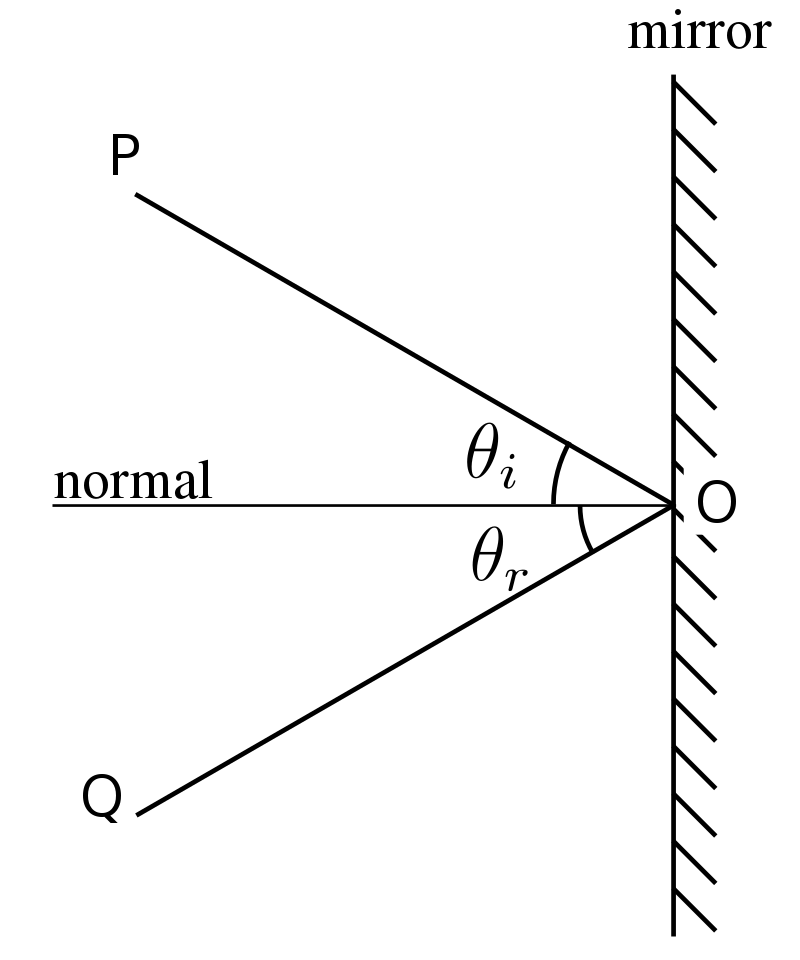
\includegraphics[width=\linewidth]{general/reflection_law.png}
    \captionof{figure}{%
        Specular reflection
    }
    \label{fig:mirage:scene}
}
% Not all the energy is reflected, part of it is absorbed.
The proportion of energy absorbed by the surface and the incident acoustic wave is measured
through the reflector's \textit{acoustic impedance}\sidenote{%
\textbf{acoustic impendence} measures the opposition that an acoustic system presents to the acoustic pressure.
}.
By relating the acoustic pressure at the reflector location with the velocity of the incoming plane waves,
one can derive the \textit{plane-wave reflection coefficient} or \textit{pressure reflector factor} $\reflCoeff$ \cite{kuttruff} as
\begin{equation}
    \reflCoeff(f, \theta) = \frac{\impedence_w(f)\cos(\theta) - \impedenceAir(f)}{\impedence_w(f)\cos(\theta) + \impedenceAir(f)}
    ,
\end{equation}
where $\impedence_w(f)$ and $\impedenceAir(f)$ are the frequency-dependent impedance of the surface and the air respectively,
and $\theta$ is the angle of incidence.

This formula holds as long as the far field assumption, namely the source, or receiver, is several wavelengths away from the infinite reflecting plane.

For the more commonly applied energy-based GA techniques,
it is customary to use the absorption coefficient a $\absCoeff$ defined as
\begin{equation}
    \absCoeff = 1 - \abs{R(f, \theta)}^2
\end{equation}






\subsection{Scattering and Diffraction}

%%%%%%%%%%%%%%%%%%%%%%%%%%%%%%%%%%%%%%%%%%%%
\section{Room Acoustic Modeling and the Room Impulse Response}
By adding boundary condition we can write the acoustic pressure within a 3-dimensional enclosure.
Let us assume the simplest possible 3-D enclosure: a cuboid room with perfectly smooth and rigid facets
\sidenote{%
\textbf{facet}: each of the plane surfaces of a polytope.
}.
More precisely, let define $\calC$ the domain of the problem as the cuboid with length $L$, width $W$ and height $H$, that is
\begin{equation}
    \calC = \kset{\positionMicrophone = (x,y,z)}{
        0 \le x \le L,\,
        0 \le y \le W,\,
        0 \le z \le Z}
\end{equation}
Let $\calB$ be the boundaries of $\calC$, \ie/ the rigid room facets.

The multiple sound propagation paths from a source to a
receiver in a room can be modeled accurately by a linear time- invariant system defined by the so-called room impulse re- sponse. A room impulse response contains several perceptu- ally relevant components


\subsection{Simulating Room Acoustics}


\subsection{the Image Source Method}
https://reuk.github.io/wayverb/context.html

\newthought{Finally} we can write the final Room Impulse Response $\rir_{ij}(t)$ as follows:
\begin{equation}
    \contMicrophoneSignal(t) = (\rir_{ij} \conv \contSource)(t)
\end{equation}

\begin{equation}
    \rir_{ij}(t) = \sum_{r=0}^{R} \frac{\alpha_r}{4 \pi \tau_r / \cair} \delta \kparen{t - \tau_r}
\end{equation}
where
\begin{itemize}
    \item $\alpha_r \in \kintervcc{0}{1}$ is the attenuation coefficient of the $r$-th reflection
    \item $\tau_r = \norm{\positionMicrophone_\idxMic - \positionSource_\idxEch}$ is the distance between the microphone and the $\idxEch$-th image of source $\idxSrc$.
\end{itemize}

\newthought{The Image Source Method}


\subsection{The Acoustic Impulse Response}

\subsection{Properties of the Room Impulse Response}
\newthoughtpar{direct path}
\newthoughtpar{early echoes}
\newthoughtpar{late reverberation}

\subsection{Room Acoustic Simulators}
https://reuk.github.io/wayverb/context.html

%%%%%%%%%%%%%%%%%%%%%%%%%%%%%%%%%%%%%%%%%%%%
\section{Acoustic Parameters and Perception}
\itodo{cite Sacks}
\newthoughtpar{The Mixing Time}
\newthoughtpar{Reverberation Time}
\newthoughtpar{Direct-to-revebrerant ratio}
\newthoughtpar{Critical Distance}
\newthoughtpar{Interchannel Coherence}
\newthoughtpar{Perception of the Early Reflection}
\newthoughtpar{Perception of the Late Reverberation}